\chapter{Réalisation}

Cette partie présente l'environnement technique, les principaux modules développés et l'intégration finale des services.


\section{Environnement de travail}

{\small\singlespacing\arrayrulecolor{tableline}
\begin{longtable}{|>{\raggedright\arraybackslash}p{\dimexpr 0.240\textwidth-2\tabcolsep-2\arrayrulewidth\relax}|>{\raggedright\arraybackslash}p{\dimexpr 0.320\textwidth-2\tabcolsep-2\arrayrulewidth\relax}|>{\raggedright\arraybackslash}p{\dimexpr 0.440\textwidth-2\tabcolsep-2\arrayrulewidth\relax}|}
\hline
\rowcolor{tablehead} \color{white}\bfseries Élément & \color{white}\bfseries Choix final & \color{white}\bfseries Rôle \\ \hline
\endfirsthead
\rowcolor{tablehead} \color{white}\bfseries Élément & \color{white}\bfseries Choix final & \color{white}\bfseries Rôle \\ \hline
\endhead
\hline\endfoot
Langage backend & Java 21 & API transactionnelle et règles métier \\ \hline
\rowcolor{tablerow} Framework backend & Spring Boot 3.2.8 & Web, sécurité, validation, JPA et WebSocket \\ \hline
Frontend & Angular 21, TypeScript 5.9 & SPA responsive et formulaires réactifs \\ \hline
\rowcolor{tablerow} Service IA & Python 3.12, FastAPI & Recherche sémantique et orchestration \\ \hline
Données & MySQL, Qdrant & Source de vérité relationnelle et index vectoriel \\ \hline
\rowcolor{tablerow} Modèle & Qwen 2.5 7B Instruct & Extraction multilingue de contraintes \\ \hline
Adaptation & Unsloth QLoRA & Entraînement local quantifié \\ \hline
\rowcolor{tablerow} Exécution LLM & Ollama & Inférence locale sur GPU \\ \hline
Tests & JUnit, Vitest, Pytest, Playwright & Validation multi-couche \\ \hline
\rowcolor{tablerow} Versionnement & Git et GitHub & Historique, partage et sauvegarde du code \\ \hline
\end{longtable}
}


\section{Backend Spring Boot}

Le backend applique une organisation par contrôleurs, services, dépôts, entités et DTO. Les contrôleurs exposent les contrats HTTP et délèguent les décisions aux services. Les DTO empêchent la sérialisation directe des entités JPA et stabilisent les données visibles. Le gestionnaire global d'exceptions transforme les erreurs en messages exploitables par Angular.


Les domaines couverts sont l'authentification, les utilisateurs, les catégories, les véhicules, les annonces, les images, les favoris, les conversations, les avis, les signalements, les recommandations et l'administration. Les événements de synchronisation avec l'IA sont publiés uniquement après la validation de la transaction ; une panne de l'index n'annule donc pas une opération légitime sur le catalogue.


\section{Frontend Angular}

L'application Angular est organisée en vues autonomes : marketplace, détail d'annonce, favoris, profil, profil public du vendeur, studio vendeur, boîte de réception et tableau de bord administrateur. La navigation et les actions changent selon le rôle. Les formulaires signalent les champs invalides et affichent les messages d'erreur retournés par l'API.


Le thème clair utilise des surfaces légèrement teintées et des accents verts et orange pour délimiter les zones, tandis que le thème sombre conserve exactement les mêmes espacements, bordures et tailles. La bascule de thème modifie seulement les variables de couleur, ce qui supprime les glissements de mise en page.


\textbf{Principe d'interface}

Une action métier importante possède toujours un état visible : chargement, succès, erreur récupérable ou confirmation. Les listes sont paginées et les filtres restent dans l'URL afin de pouvoir revenir à la même recherche.


\section{Captures de l'application finale}

Les captures suivantes ont été produites sur l'application Angular exécutée localement. Les données affichées proviennent d'un jeu de démonstration déterministe conforme aux contrats de l'API ; elles permettent de documenter les principaux parcours sans exposer de coordonnées ni de conversations réelles.

\begin{figure}[H]
\centering
  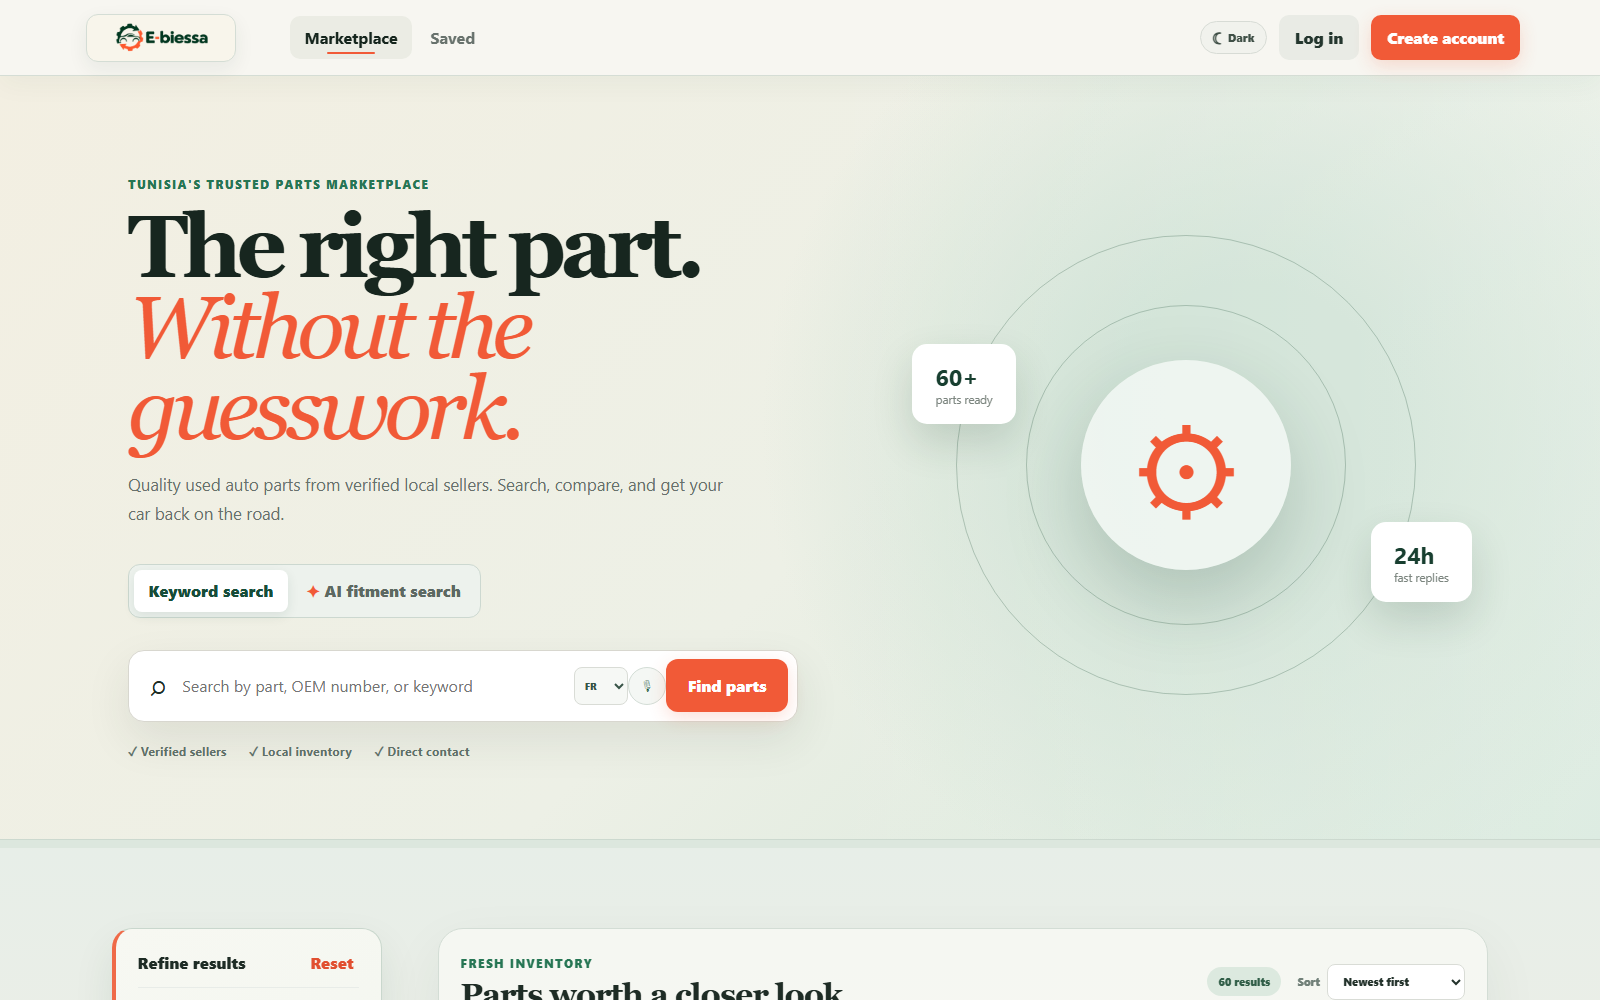
\includegraphics[width=\textwidth]{ui-marketplace.png}
\caption{Page d'accueil et accès à la recherche du marketplace E-biessa.}
\label{fig:ui-marketplace}
\end{figure}

\begin{figure}[H]
\centering
  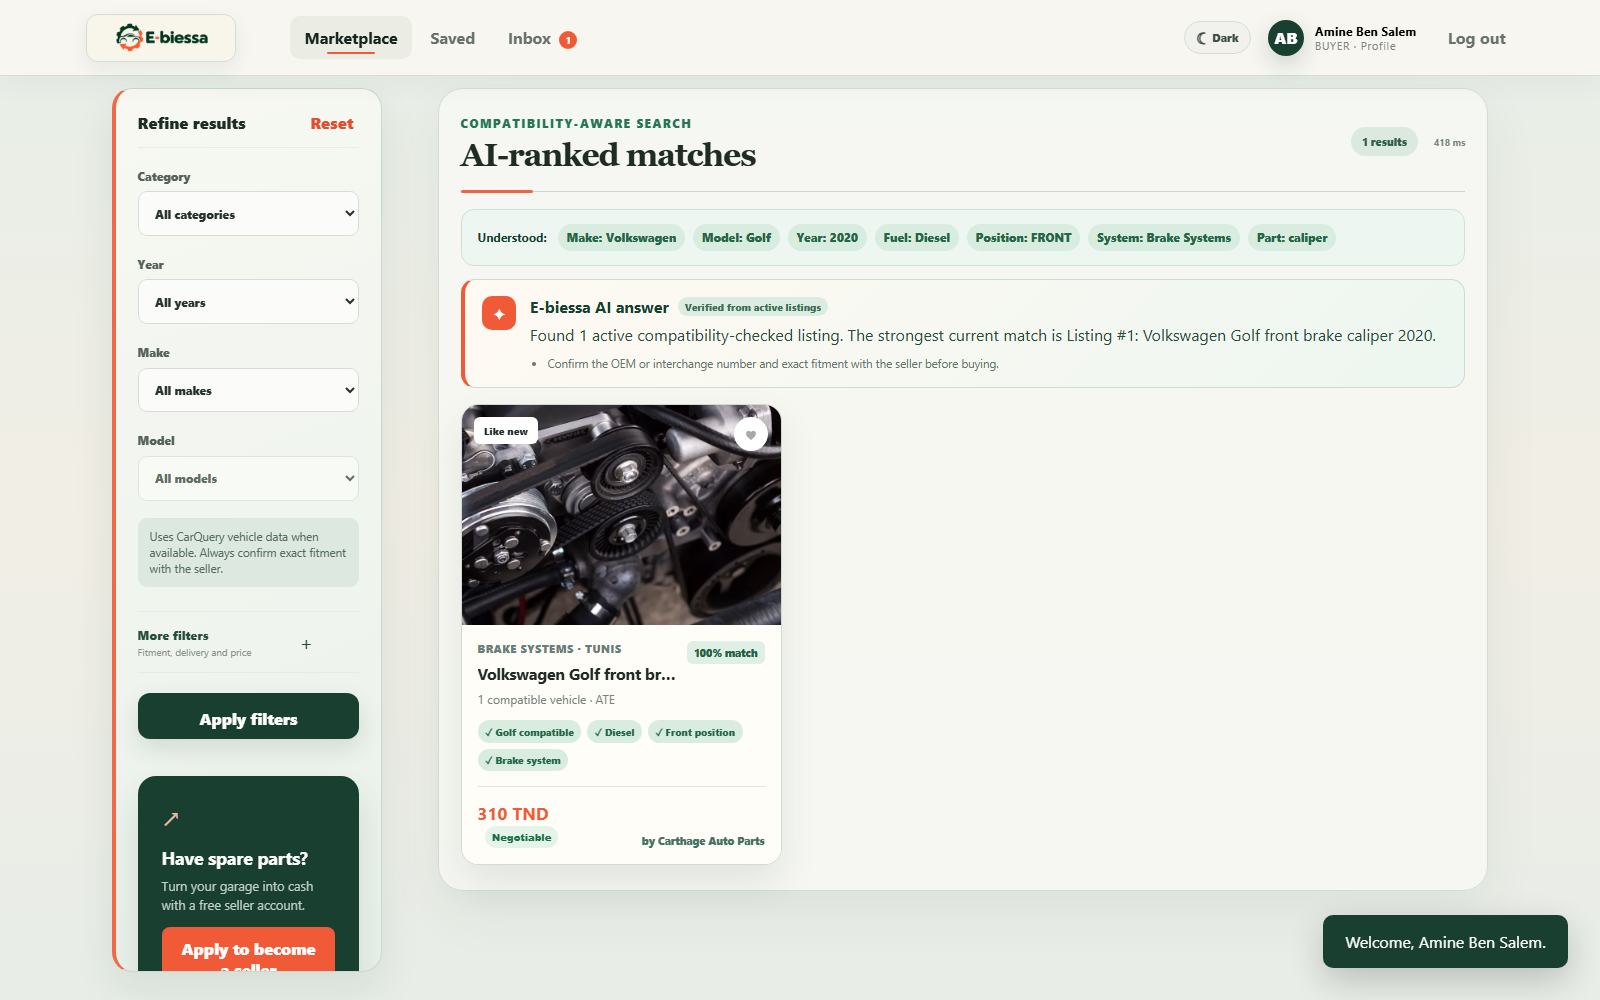
\includegraphics[width=\textwidth]{ui-ai-search.png}
\caption{Recherche IA avec contraintes extraites, réponse déterministe et explications de compatibilité.}
\label{fig:ui-ai-search}
\end{figure}

\begin{figure}[H]
\centering
  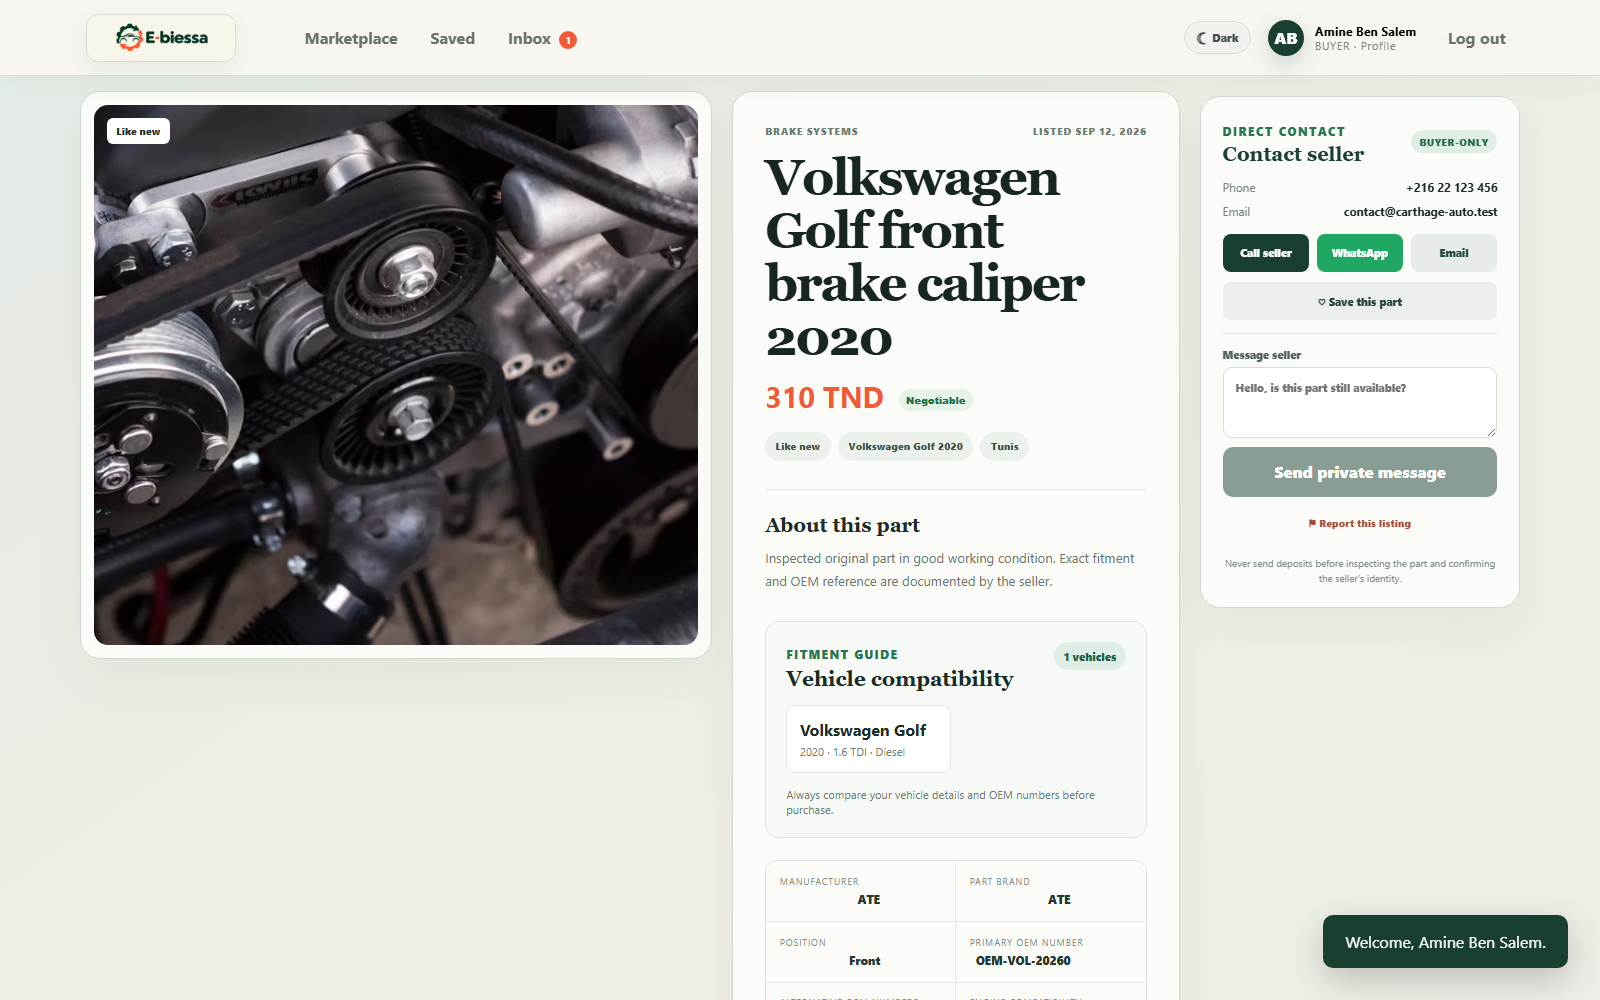
\includegraphics[width=\textwidth]{ui-listing-detail.png}
\caption{Fiche détaillée d'une pièce : compatibilité véhicule et contact vendeur protégé.}
\label{fig:ui-listing-detail}
\end{figure}

\begin{figure}[H]
\centering
  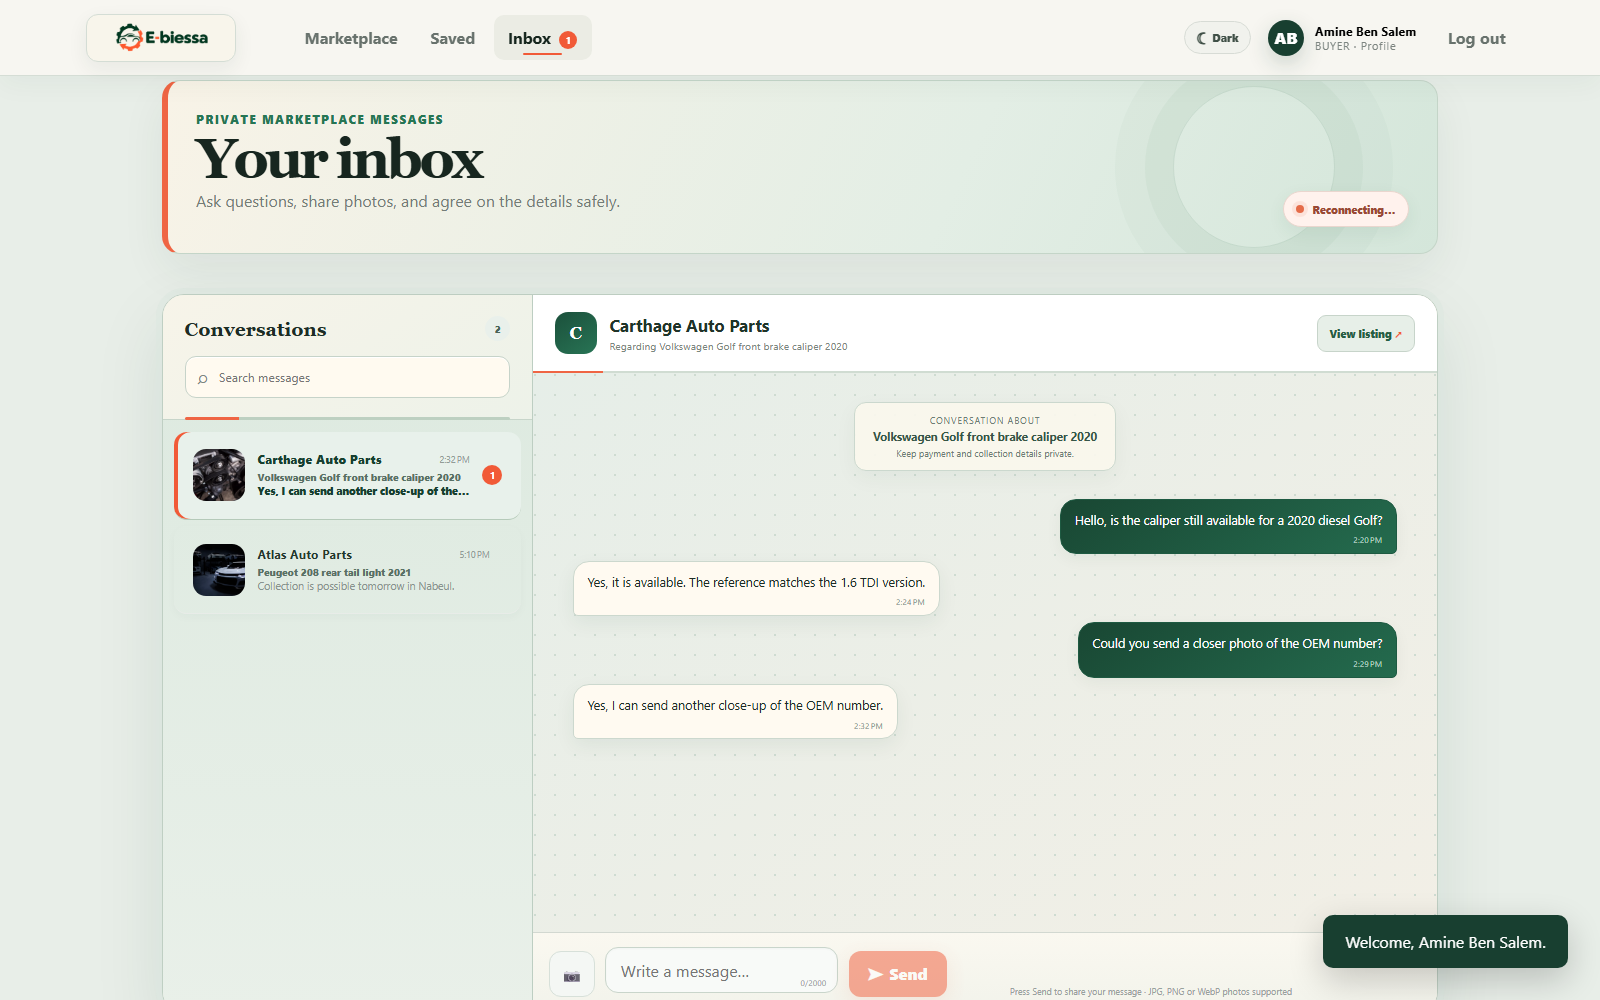
\includegraphics[width=\textwidth]{ui-messaging.png}
\caption{Boîte de réception et conversation privée entre acheteur et vendeur.}
\label{fig:ui-messaging}
\end{figure}

\begin{figure}[H]
\centering
  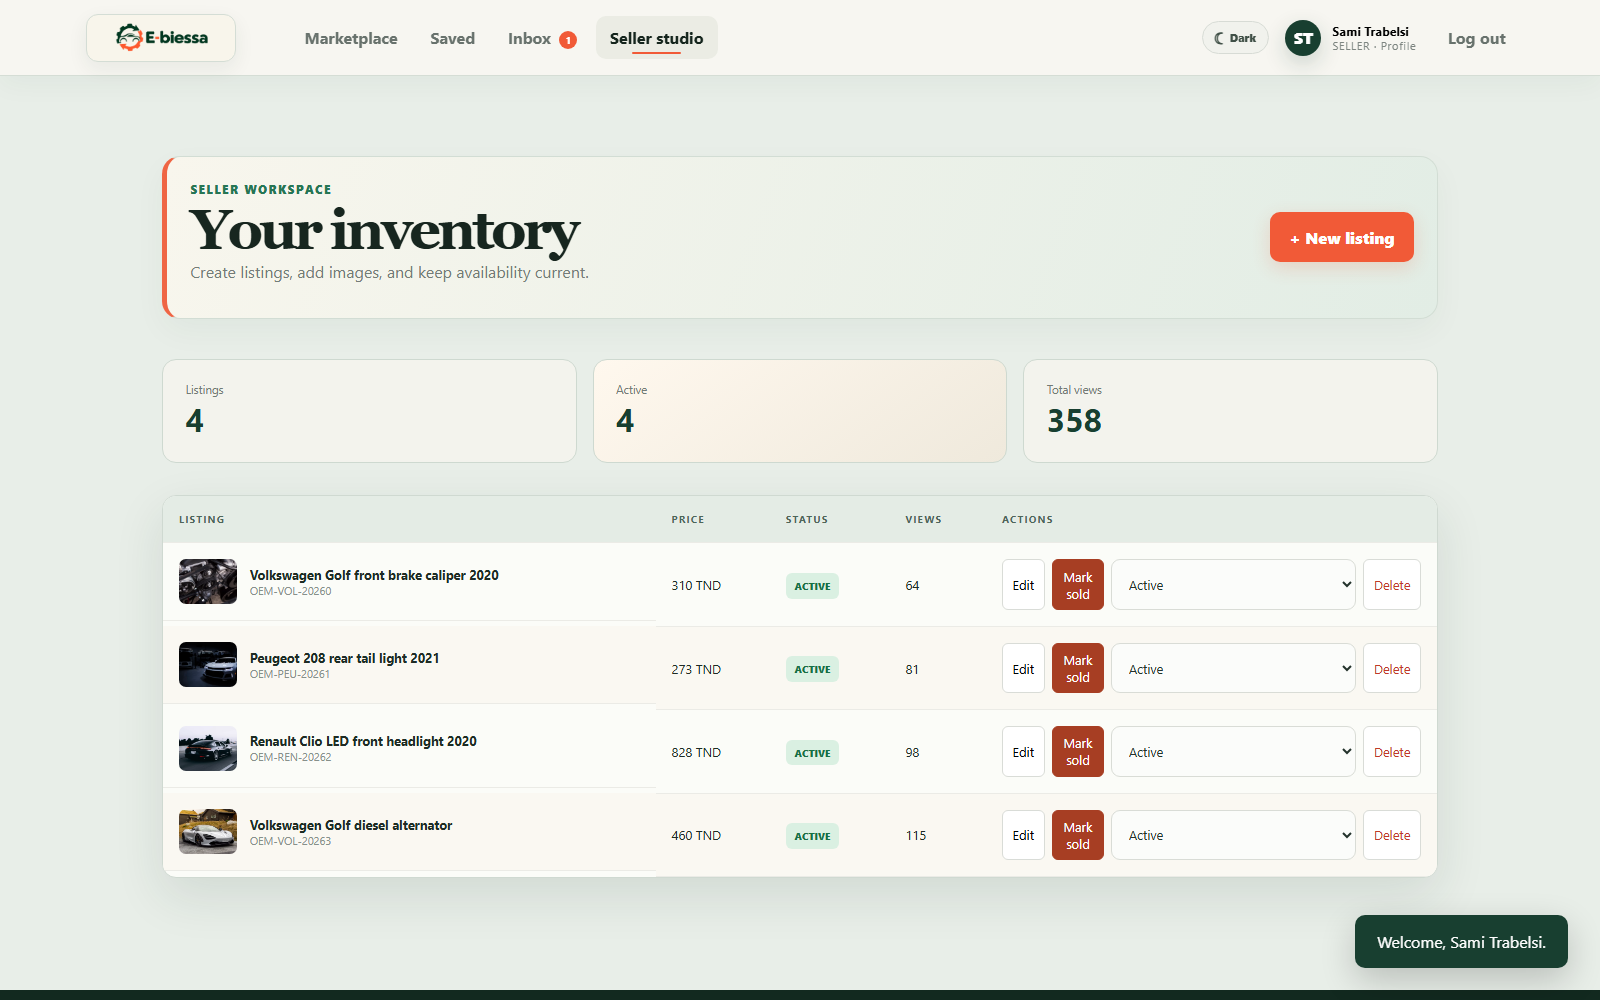
\includegraphics[width=\textwidth]{ui-seller-studio.png}
\caption{Studio vendeur pour le suivi des annonces, des statuts et des vues.}
\label{fig:ui-seller-studio}
\end{figure}

\begin{figure}[H]
\centering
  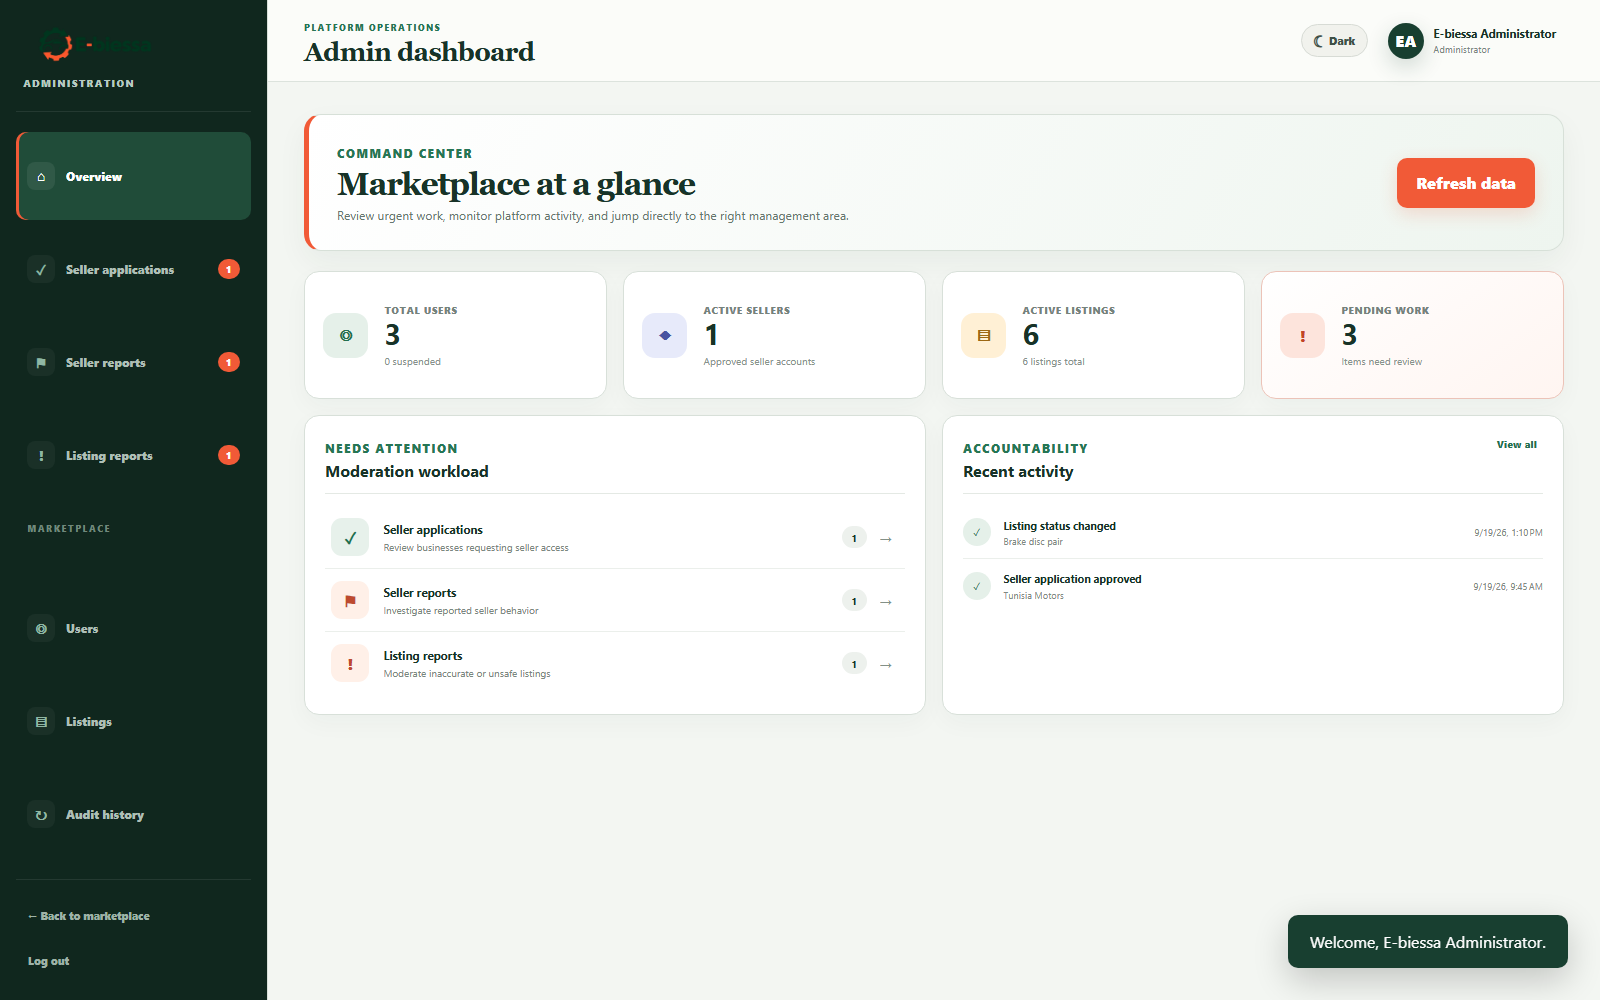
\includegraphics[width=\textwidth]{ui-admin-dashboard.png}
\caption{Tableau de bord administrateur et synthèse des files de modération.}
\label{fig:ui-admin-dashboard}
\end{figure}


\section{Gestion complète des annonces}

{\small\singlespacing\arrayrulecolor{tableline}
\begin{longtable}{|>{\raggedright\arraybackslash}p{\dimexpr 0.350\textwidth-2\tabcolsep-2\arrayrulewidth\relax}|>{\raggedright\arraybackslash}p{\dimexpr 0.650\textwidth-2\tabcolsep-2\arrayrulewidth\relax}|}
\hline
\rowcolor{tablehead} \color{white}\bfseries Bloc & \color{white}\bfseries Informations prises en charge \\ \hline
\endfirsthead
\rowcolor{tablehead} \color{white}\bfseries Bloc & \color{white}\bfseries Informations prises en charge \\ \hline
\endhead
\hline\endfoot
Identification & Titre, description, catégorie, fabricant, marque de pièce, OEM principal et alternatives \\ \hline
\rowcolor{tablerow} État commercial & Prix, négociable, état, garantie, livraison, collecte et localisation \\ \hline
Compatibilité & Plusieurs véhicules, année, moteur, carburant et position \\ \hline
\rowcolor{tablerow} Médias & JPEG/PNG/WebP, compression, ordre, image principale et suppression \\ \hline
Cycle de vie & Aperçu avant envoi ; états ACTIVE, INACTIVE, SOLD ; suppression séparée \\ \hline
\rowcolor{tablerow} Découverte & Filtres, tri, pagination, favoris, recherche IA et recommandations \\ \hline
\end{longtable}
}


\section{Comptes, profils et confiance}

L'identité locale est liée à l'adresse électronique et peut être complétée par Google, Facebook ou Microsoft lorsque les identifiants OAuth correspondants sont configurés. Le profil séparé contient nom, téléphone, localisation, nom commercial, site web et biographie. L'acheteur qui souhaite vendre soumet ces informations ; son statut reste en attente jusqu'à la décision d'un administrateur.


Un acheteur ayant déjà ouvert une conversation avec un vendeur peut lui attribuer de une à cinq étoiles et ajouter un commentaire facultatif. Un seul avis est conservé par couple acheteur--vendeur et peut être mis à jour. Cette condition atteste un contact, pas un achat confirmé : aucune commande payée n'est enregistrée dans la plateforme. La moyenne et le nombre d'avis sont publics. Les signalements et leur résolution administrative sont gérés séparément.


\section{Contact et messagerie}

La fiche annonce comporte une section « Contacter le vendeur ». Pour réduire l'extraction automatisée, les coordonnées ne sont renvoyées qu'à un acheteur connecté. Les boutons génèrent un appel téléphonique, un message WhatsApp préparé avec le titre de la pièce ou un courriel. L'acheteur peut aussi démarrer une conversation interne.


La boîte de réception présente une liste organisée de conversations et un panneau de discussion. Le fil possède une hauteur limitée, s'ouvre sur le dernier message et conserve le défilement vers les anciens échanges. L'envoi d'une image permet au vendeur de fournir des vues supplémentaires d'une pièce sans exposer un canal externe.


\section{Mise en oeuvre de l'IA}

Le modèle de base Qwen 2.5 7B Instruct a été chargé en 4 bits puis adapté avec Unsloth et LoRA de rang 8 sur un ordinateur équipé d'une RTX 4060 de 8 Go de VRAM et de 16 Go de mémoire système. Le jeu d'apprentissage contient des formulations anglaises, françaises et tunisiennes ainsi que les sorties JSON canoniques attendues. Une passe d'entraînement a été retenue après un test court, car les erreurs restantes concernaient surtout la copie de chiffres et relevaient mieux d'une validation déterministe que d'époques supplémentaires.


Le corpus corrigé v2 comprend 1 120 exemples d'apprentissage, 160 de validation et 120 de test. Les fichiers d'évaluation sont conservés séparément. La configuration locale limite la séquence à 256 tokens, utilise un lot de taille 1 et accumule les gradients sur huit étapes. Le taux d'apprentissage retenu pour l'époque v2 est de 0,00005.


Le modèle exporté est servi localement par Ollama sous le nom e-biessa-query-v2. FastAPI lui demande uniquement un objet structuré. La fonction de fusion contrôle ensuite l'année explicite, normalise les catégories et vérifie chaque valeur dans le catalogue. Cette approche apporte la souplesse linguistique du LLM tout en gardant un comportement reproductible.


\section{Jeu de démonstration}

Le profil de développement initialise un administrateur, trois acheteurs, trois vendeurs et soixante annonces réparties entre plusieurs marques, modèles, catégories et villes. Chaque vendeur possède plusieurs annonces détaillées. Les données sont réutilisables sans duplication au redémarrage et servent uniquement à la démonstration académique.


{\small\singlespacing\arrayrulecolor{tableline}
\begin{longtable}{|>{\raggedright\arraybackslash}p{\dimexpr 0.350\textwidth-2\tabcolsep-2\arrayrulewidth\relax}|>{\raggedright\arraybackslash}p{\dimexpr 0.650\textwidth-2\tabcolsep-2\arrayrulewidth\relax}|}
\hline
\rowcolor{tablehead} \color{white}\bfseries Donnée & \color{white}\bfseries Volume de démonstration \\ \hline
\endfirsthead
\rowcolor{tablehead} \color{white}\bfseries Donnée & \color{white}\bfseries Volume de démonstration \\ \hline
\endhead
\hline\endfoot
Administrateurs & 1 \\ \hline
\rowcolor{tablerow} Acheteurs & 3 \\ \hline
Vendeurs & 3 \\ \hline
\rowcolor{tablerow} Annonces actives initiales & 60 \\ \hline
Définitions véhicule locales & 20 \\ \hline
\rowcolor{tablerow} Langues d'exemple IA & anglais, français, arabe tunisien translittéré \\ \hline
\end{longtable}
}


\section{Configuration et exécution locale}

1. Démarrer MySQL et créer la base marketplace.


2. Définir les variables DB\_URL, DB\_USERNAME, DB\_PASSWORD, JWT\_SECRET et CORS\_ALLOWED\_ORIGINS dans l'environnement local de Spring.


3. Définir le même AI\_SERVICE\_TOKEN dans Spring et FastAPI, puis activer l'intégration IA.


4. Lancer Ollama avec le modèle adapté e-biessa-query-v2.


5. Démarrer FastAPI sur 127.0.0.1:8001, Spring Boot sur localhost:8080 et Angular sur localhost:4200.


6. Exécuter une réindexation complète avec le compte administrateur avant la première recherche sémantique.


\section{Assistance VIN et catalogue automobile}

Le profil acheteur propose la saisie d'un VIN de 17 caractères. Spring contrôle le format, interroge NHTSA vPIC puis rapproche la marque, le modèle, l'année et le carburant des lignes Vehicle du catalogue local. L'interface propose uniquement les identifiants locaux reconnus ; l'acheteur doit confirmer l'enregistrement de ses préférences. Une absence de correspondance conduit à la sélection manuelle, sans création automatique d'une compatibilité.


Le décodage utilise un délai configuré et un cache temporaire, fixé par défaut à 24 heures. Le VIN n'est pas persisté en base ; il est néanmoins transmis à NHTSA et intervient dans le cache de requête. La couverture vPIC, principalement orientée vers le marché américain, limite la reconnaissance de certains véhicules européens ou tunisiens. Le décodage n'est jamais présenté comme une garantie de montage.


\section{Estimation indicative du prix}

PriceEstimatorService compare la saisie du vendeur à un maximum de vingt annonces actives. Le score tient compte de la référence OEM, de la catégorie, des véhicules partagés, des termes du titre, de la position, de la marque de pièce et de l'état. L'annonce en cours d'édition et les vendeurs suspendus sont exclus. En l'absence de comparables suffisants, le système ne fabrique pas de prix.


La réponse fournit un prix central, une plage interquartile, le nombre de comparables et un niveau de confiance heuristique. Les quantiles de l'implémentation correspondent au rang arrondi dans la liste triée ; pour un effectif pair, le prix central n'est donc pas nécessairement la moyenne des deux valeurs centrales. Le calcul porte sur des prix demandés, pas sur des ventes conclues. Le vendeur conserve la décision et doit explicitement appliquer la suggestion.


\section{Identification de pièces par image}

L'utilisateur connecté peut transmettre une image JPEG, PNG ou WebP, limitée à 5 Mo. Spring applique l'authentification, la limitation de débit et les validations avant de transmettre les octets au service FastAPI avec le jeton interne. Le module optionnel utilise openai/clip-vit-base-patch32 pour comparer l'image à une taxonomie de vingt-deux types de pièces et retourner au plus cinq candidats.


Il s'agit d'une classification zero-shot, distincte de l'adaptation QLoRA de Qwen. Les scores sont relatifs aux catégories proposées, et non des probabilités calibrées de justesse. Le système ne déduit ni véhicule exact, ni référence OEM, ni garantie de compatibilité à partir des pixels. Le candidat choisi alimente une recherche dont les règles déterministes restent actives.


VISION\_ENABLED reste désactivé par défaut. L'activation requiert les dépendances de vision et le téléchargement initial du modèle, mis en cache pour les requêtes suivantes. Aucune fonction métier ne conserve la photo d'identification ni ne l'utilise pour l'apprentissage ; le traitement multipart peut toutefois recourir à des fichiers temporaires selon la configuration du serveur. Les tests automatisés isolent l'inférence au moyen d'un substitut.


\section{Saisie vocale}

Angular exploite la reconnaissance vocale proposée par le navigateur avec un choix français de Tunisie, arabe de Tunisie ou anglais américain. Le texte reconnu reste modifiable et la recherche ne part qu'après confirmation. L'absence de microphone, le refus de permission ou l'absence de prise en charge laisse disponible la saisie au clavier.


E-biessa reçoit la transcription, pas l'enregistrement audio. Le navigateur peut cependant faire appel au service vocal de son fournisseur ; la fonctionnalité ne doit pas être décrite comme une reconnaissance entièrement locale. Les tests utilisent un objet de reconnaissance simulé ; la qualité acoustique dépend d'une vérification réelle sur le navigateur et le microphone retenus.
